%%This is a very basic article template.
%%There is just one section and two subsections.
\documentclass[UTF8]{ctexart}
\title{第三章 SerDes接收端整体结构介绍}
\author{陈登}
\date{\today}

\bibliographystyle{plain}
\usepackage{graphicx}
\usepackage{float}
\usepackage{amsmath}
\usepackage{geometry}
\usepackage{fontspec}
\usepackage{algorithm}
\usepackage{algorithmicx}
\usepackage{algpseudocode}

\geometry{a4paper,centering,scale=0.9}
\usepackage[format=hang,font=small,textfont=it]{caption}
\usepackage[toc,page,title,titletoc,header]{appendix} 
\usepackage[nottoc]{tocbibind}

\begin{document}

\section{SerDes接收端整体结构介绍}

\subsection{总体框架}

JESD204B协议能够支持多Converter\footnote{Converter即为一个模数或者数模转换器,在本文中代指单个数字样本的数据流接口。}、多link\footnote{link即为数据连接。}、多lane\footnote{lane即为同一方向的单个差分信号对。}的数据传输,并且不同设备之间允许采用不同的时钟,实现异步传输。
基于JESD204B协议的传输结构图如图\ref{fig:jesd204b_stuct}所示。

\begin{figure}[H]
\centering
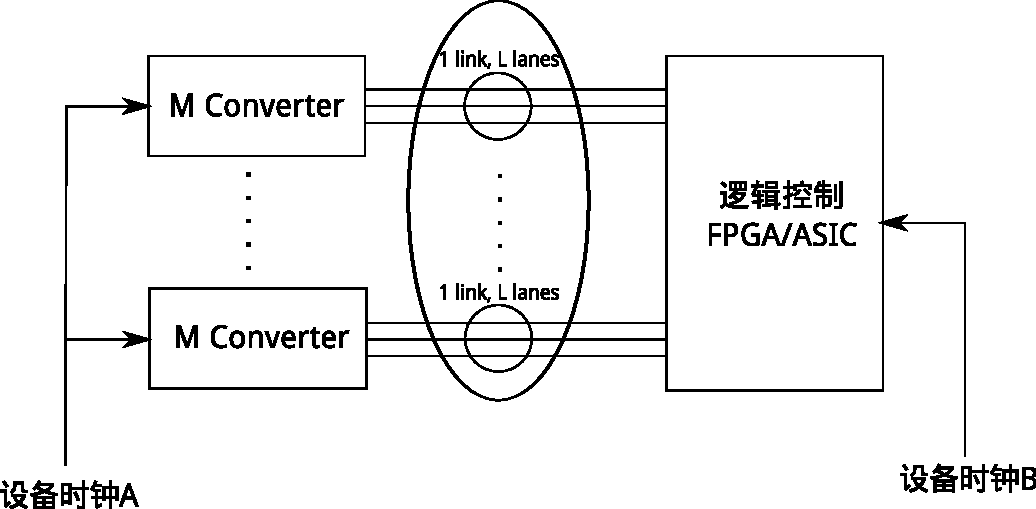
\includegraphics[width=10cm]{./img/jesd204b_stuct.pdf}
\caption{JESD20B协议传输结构框图}
\label{fig:jesd204b_stuct}
\end{figure}

基于JESD204B协议的SerDes接收端在数据流传输上,主要包括了数据链路层协议和传输层协议,并且为了实现这两个层面的协议,定义了一系列配置寄存器,供使用者配置SerDes接收端。
数据流传输结构框图如图\ref{fig:serdes_sturct_link_transport_layer}所示。

\begin{figure}[H]
\centering
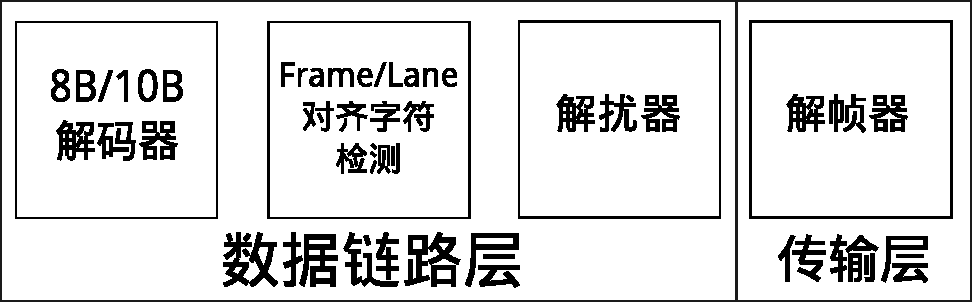
\includegraphics[width=10cm]{./img/serdes_sturct_link_transport_layer.pdf}
\caption{SerDes接收端数据流传输结构框图}
\label{fig:serdes_sturct_link_transport_layer}
\end{figure}

在实际使用中的SerDes接口接收端还包含有Crossbar Mux用来将物理lane端口,对应到逻辑lane端口,使得端口的使用配置更加灵活。
发送端在发送数据时,为保证传输的数据能够适应信道的特性,降低误码率,对原始信号进行了编码和加扰;又为了保证接收端能够正确的识别出恢复出的信号属于哪一个时刻哪一个设备,添加了控制信息、帧定界符等具体信息。
数据链路层主要的功能就是对由物理层获得的码流进行初步的解析,进行解码和解扰的操作,恢复出实际的传输数据。
同时也对以一个字符为单位的frame和lane进行对齐校验,以保证时序正确。
传输层主要的功能就是对由数据链路层解析出来的码流进行解帧操作,恢复到传输前的具体信息,对应到相应的设备、converter等。

\subsection{数据链路层}

数据链路层是物理层获得码流后首个进入的数据逻辑层面,该层面主要负责对数据流进行解码、解扰、帧检测以及同步的工作。

JESD204B协议规定了8B/10B编码作为数据链路层的编码,该编码主要参照IEEE802.3以太网协议中的8B/10B编解码标准。
在以太网标准的基础上,JESD204B协议也做了一定的取舍,只采取了协议中一部分控制码字作为SerDes传输的控制码字。
采用这种编码方式主要有以下几点优势:

\begin{itemize}
\item 传输密度均匀,能够使得时钟恢复更加便利。
\item 编码中含有足够数量的控制字,利于数据帧的构建。
\item 能够直接通过控制字标示出frame的开始和结束。
\item 能够直接通过控制字标示出alignment,区分出各个lanes。
\item 该编码是直流平衡的编码,便于有线信道传输,降低功耗,减小误码率。
\item 根据编码的顺序特性,能够一定程度上检测到错误的码字。
\end{itemize}

JESD204B协议也规定了几种同步方式,使得接收到的数据流能够保证时序上的正确。
包括码群同步\footnote{Code Group Synchronization}、初始化frame同步\footnote{Initial Frame Synchronization}、初始化lane同步\footnote{Initial Lane Synchronization}。
码群同步的主要目的是在最初的连接发起阶段,通过发送数个固定码字/K28.5/控制字,使接收端快速跟踪到发送端的时钟,通过始终恢复电路完成对齐工作,保证接下来的传输稳定。
在完成码群同步后,就需要发送一个关键的初始化lane对齐序列\footnote{Initial Lane Alignment Sequence,即ILAS。},在这个帧中包含了本次通信的具体配置信息,接收端要根据这个帧的内容和实际的由寄存器设置的配置内容,完成对接收端的设置。
初始化frame同步的主要目的是对frame进行同步,同时进行frame同步的监测、纠错功能。
初始化frame同步主要通过监视数据流中frame对齐字符实现,这些对齐字符是由发射端在确定情况下加在每一个frame的结尾处。
通过配置信息以及frame对齐字符的位置,可以推断出接收端是否跟踪上frame同步,若发现未跟踪上同步则需要及时报错并通知发送端。
初始化lane同步主要是通过对齐字符保证各个lane同步的被接收到,通过接收端来对齐。
各条lane基本上表示各条差分传输对,每一个converter所使用的lane需要对齐就由初始化lane同步来确保。
当所有接收端标示了对齐接收到的标志后,则同时向上层传输收到的数据。

加扰和解扰技术是串行通信中经常使用的关键技术,目的就在于增加传输数据的随机性,避免过多的连续字符出现,影响传输效果。
串行加解扰可分为同步扰码和自同步扰码,两者的区别在于输入到反馈移位寄存器的序列不同,自同步扰码由之前传输序列决定,同步扰码则需要另外干预。
同步扰码的实质是让输入比特再与随机数产生器所共同产生的随机位进行异或来产生扰码的确定输出。
在JESD204B协议规定中,加解扰采用的是自同步机制,并且加扰和解扰是可选项,可以通过寄存器配置取消或使用加解扰技术,增加了传输的灵活性。
一般加扰技术应用于编码和成帧之前,解扰在解码和同步之后,并且加解扰是根据具体加解扰公式确定,需要根据前一组数据的情况才能计算出下一组数据的加扰后值。
所以有一个字符的延时,接收端要在正确收到一个字符后才能对下一个字符正确的解扰,往往在启用加解扰之后的第一个传输的字符是不进行加扰和解扰的。
加解扰位置如图\ref{fig:functional_location_of_scrambler_and_descrambler}所示。

\begin{figure}[H]
\centering
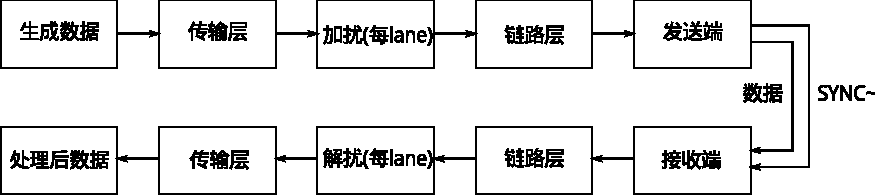
\includegraphics[width=15cm]{./img/functional_location_of_scrambler_and_descrambler.pdf}
\caption{加解扰结构位置示意图}
\label{fig:functional_location_of_scrambler_and_descrambler}
\end{figure}

\subsection{传输层}

传输层是数据流经过数据链路层解码、解扰、同步之后将数据流重新恢复为模数转换器数据的层面,这一层面的主要作用就是根据配置规定,提取出相关转换器的数据。

JESD204B协议主要支持以下几种成帧方式,这也是接收端需要负责完成解帧的几种格式:

\begin{itemize}
\item 单个设备单个converter到单个lane的link。
\item 单个设备多个converter到单个lane的link。
\item 单个设备单个converter到多个lane的link。
\item 单个设备多个converter到多个lane的link。
\end{itemize}

以上成帧方式,是直接定义在协议中的,可以发现JESD204B协议主要还是针对单个设备的连接协议。
但在单个设备中可以存在单个或者多个converter,即模数或数模转换器。

在实际传输中,一系列的样本或者部分样本组成一个frame\footnote{frame,即一组连续的octet。一些位置的octet可以被用作frame对齐信号。},一个frame可以包含F\footnote{F,即表示每个frame的octet数量。}个octet\footnote{octet,即8位二进制数据}。
并且在大部分实现中,frame的时钟频率和采样频率相同。
协议允许在每个frame周期中,同一个converter传送多个样本,样本的数量由寄存器配置项S\footnote{S,单个converter每个frame周期传输的样本数。}决定。
每一个样本就是一组编码,由可以控制的变量N\footnote{N,即converter的分辨率}来决定样本的位数,并且允许包含控制位和结束位。

考虑最复杂情况,即多个converter,多个lane的成帧情况,成帧方式如图\ref{fig:user_data_format_for_multiple_lanes}所示。其中M表示单个设备converter的数量,CF表示每个link中每个frame时钟周期控制字的数量,NG表示4位长度二进制数据,L表示每个设备的lane数。

\begin{figure}[H]
\centering
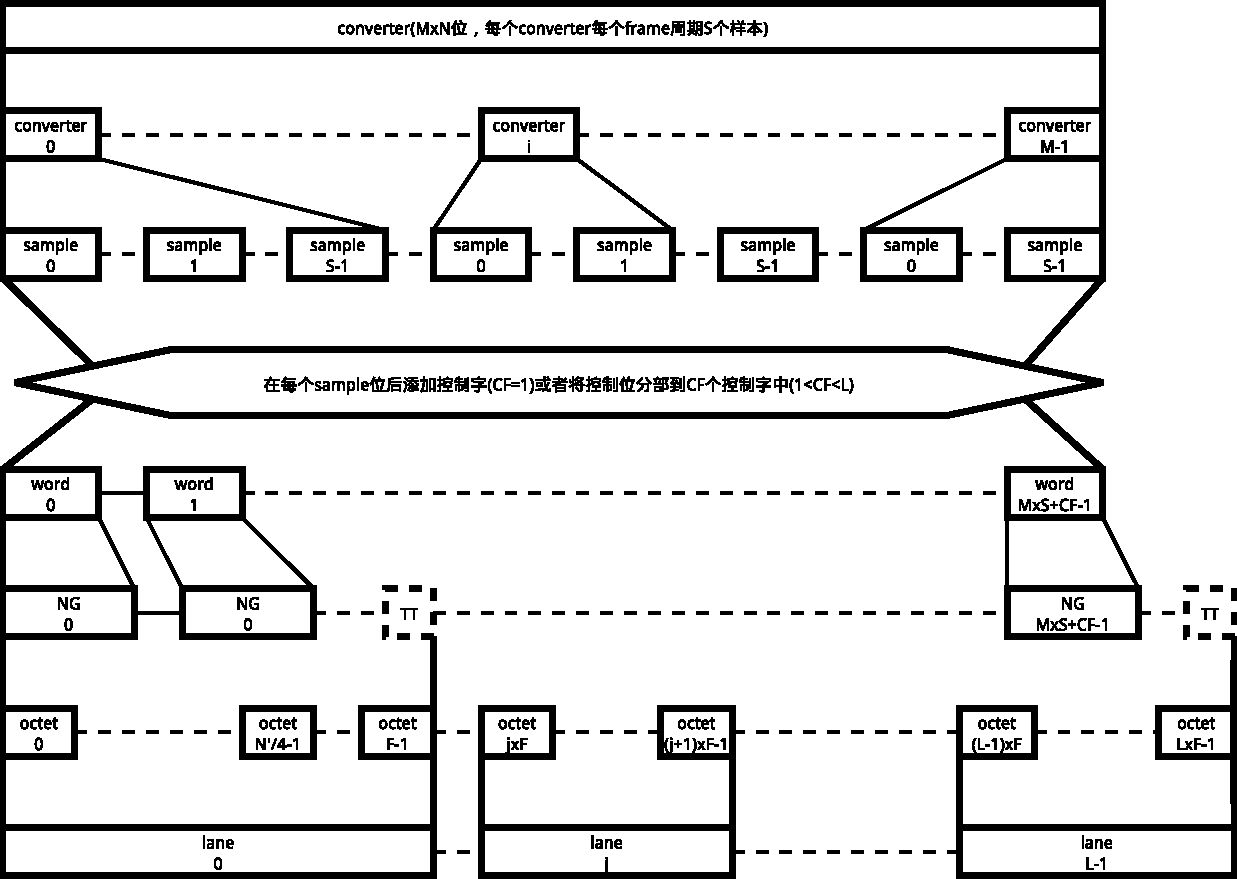
\includegraphics[width=17cm]{./img/user_data_format_for_multiple_lanes.pdf}
\caption{多lane传输的用户数据格式}
\label{fig:user_data_format_for_multiple_lanes}
\end{figure}

\subsection{设计指标}

本文的设计旨在一定的工艺库支持及约束条件下,设计出符合JESD204B协议规范的SerDes接收端传输层和数据链路层。

第一个重要的实现目标就是多版本兼容。
JESD204B协议是JESD204协议经由JESD204A协议的升级版本,增加了许多新的功能和特性,尤其是在多设备通信和固定时延设计上。
协议规定了需要支持的三个Subclass,其中Subclass 0即表示JESD204协议,Subclass 1即表示JESD204A协议,Subclass 2即表示最新的JESD204B协议。
设计中需要配有相应的寄存器来选择对应的Subclass,只有当收发端都为相同的Subclass时才能正确通信。

第二个是设计达到的层级。
本设计的设计范围是接收端的传输层和数据链路层,相应的设计层级是门级综合,即能根据特定工艺库生成门级网表。
设计的流程即为RTL级逻辑代码,到RTL级仿真,最后到门级综合。

第三个是具体性能指标。
芯片设计的性能指标主要包括功耗、面积、时序、工作频率等。
这些都受限于所采用的工艺库和约束条件,所以以下讨论均采用SMIC180工艺,布线负载采用wl10。
本设计主要运用于高端的模数、数模转换芯片,并主要使用在无线通信的基站端,对于功耗的要求相对较低,所以在保证性能的前提下不会着重考虑功耗的问题。
但由于是整个芯片中比较小的功能模块,所以对面积有一定的要求,设计需要限制在器件面积10000$\mu m^2$以内(不包括布线面积)。
最后是工作频率,高速的通信芯片需要能够达到较高工作频率,但是受限于工艺,设计需要限制在500$Mhz$。

\bibliography{../../bib/serdes}
\end{document}

